\chapter{序論} % 章のタイトル

% \includegraphics[width=??cm]{hoge.eps} % 図(EPS形式)を読み込む場合

\section{背景} % sectionのタイトル

% 以下に背景,関連する環境状況,技術に関する概要を記述.

近年,インターネット技術やセンサー技術の進化を背景に,パソコンやスマートフォンなどのインターネット端末に加え,家電や自動車などの様々なものに通信機能を搭載したIoTデバイスが普及し始めている.総務省によると政界中のIoTデバイスの数は図1のように2017年時点でIoTデバイスが約275億台存在し,2020年にはIoTデバイスが403億台に及ぶと予想されている\cite{IoT}.
 \begin{figure}[h]
 \centering
    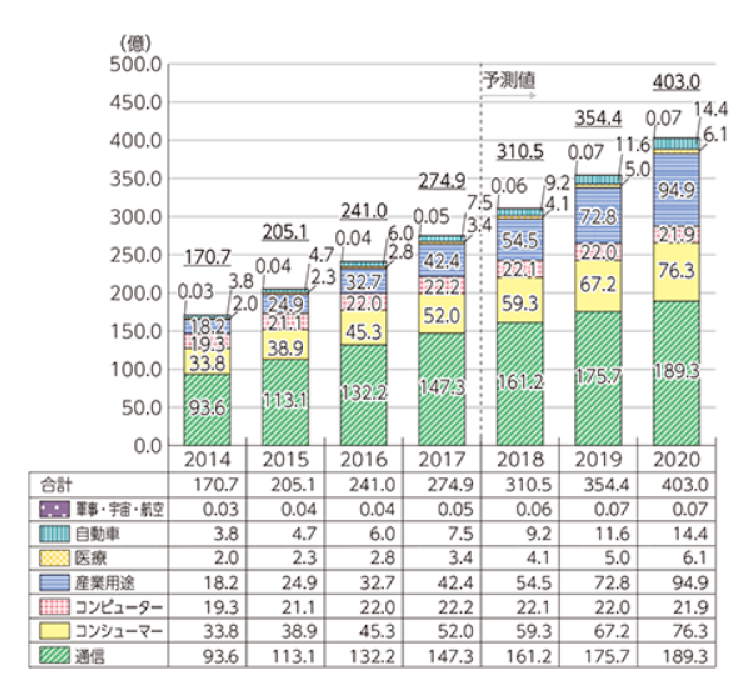
\includegraphics{figures/IoT_device.eps}
 \label{fi:model}
 \begin{center}図1 世界のIoTデバイス数の推移及び予測\end{center}
 \end{figure}
IoTデバイスの普及に伴い,IoTデバイスを対象としたマルウェアが急増している.
IoTデバイスの重要な問題の1つとしてセキュリティ問題が挙げられる.IoTデバイスのユーザ名やパスワードを初期設定の状態で使用する場合が多いことやデバイスの資源が限られていることから,セキュリティが十分に考慮されていない事がある.そのため,IoTデバイスを対象としたマルウェアが脅威となっている.その中でもネットワークサービスを停止させる深刻な問題を引き起こしているマルウェアにはDDoS(Distributed Denial of Service)攻撃を行っているものが多く存在し,その対策が重要視されている.DDoS攻撃は,攻撃者が複数の他人のコンピュータを利用し,公開されているサービスに大量のデータを送りつける事によって処理負荷を与えサービスを機能停止に追い込む攻撃である.代表的なDDoS攻撃を行うマルウェアとしてMiraiが挙げられる.Mirai\cite{Mirai}では,無作為なIPアドレスから感染できるデバイスを探し出し,ログイン可能なデバイス上に,悪意のあるソフトウェアをダウンロードし実行させることでそのデバイスを制御下に置く.攻撃者によって制御された端末は他に侵入可能な端末を探し出し,次々と感染させることでボットネットと呼ばれる悪意あるプログラムを使用して乗っ取った多数のコンピュータで構成されるネットワークを構築する.その後,C\&C(Command and Control)サーバから送られた指示に対してDDoS攻撃を行うマルウェアである.2016年10月に発生した,DNSサーバープロバイダであるDyn社へのDDoS攻撃ではIoTデバイスによるボットネットが利用され史上最大規模である620Gbpsの攻撃が観測された\cite{Dyn}.その後,Miraiのソースコードが公開され,Owari,Satori,OkiruといったMiraiの亜種の開発が盛んに行われるようになった.マルウェアに基づいて作成されたデータを用いたパターンマッチングによる検知手法では,誤検知率が低く既存のマルウェアを確実に検知できる利点が有る.公開されているソースコードを基に作成されたマルウェアは,オリジナルのマルウェアと共通するシグネチャが存在すると考えられるためパターンマッチングによる検知で亜種のマルウェアにも対応できると想定される.脅威となっているマルウェアは,十分に管理が行われていないIoTデバイスで散見される,放置された初期パスワードのままのアカウントや,保守されていないシステムの脆弱性をついた攻撃を行うため,侵入されてしまうことは前提とすべきである.そのため,デバイスの性能が限られているIoTデバイス上でもマルウェアの検知を行う必要がある.

\section{対象とする領域}

実用レベルのサイズのプログラムを作成するためのプログラミング言語につい
て研究する.ここで,行うのは3次元グラフィックス向けの言語の設計とその
インタプリタの実装である.

\section{研究目的}

本研究では,DDoS攻撃を行うマルウェアMiraiとその亜種の未知のマルウェア検知である.
